% ============================================================
%  SECTION IV — LEAK AUDIT AND DATASET VALIDATION
%  SECTION V  — BASELINE EXPERIMENTS
%  \input'd from main.tex
% ============================================================

% ------------------------------------------------------------------
\section{Leak Audit and Dataset Validation}
\label{sec:audit}
% ------------------------------------------------------------------

Before any detector is trained on \textbf{\datasetname}, it is
necessary to verify that the preprocessing pipeline actually eliminates
the known sources of shortcut learning, and that no structural
artefact distinguishes the two classes for reasons unrelated to
synthesis.
We conduct this verification in three steps: a canonical-format
audit, a SHA-256 integrity check, and a one-epoch
\emph{sniff test}~\cite{grommelt2024jpeg} using a deliberately weak
detector.

\subsection{Canonical-Format Audit}
\label{ssec:audit_format}

Every image stored in the repository is validated against the
\texttt{png\_is\_canonical} predicate (described in
Section~\ref{ssec:preprocess}).
The predicate rejects any image that is not a PNG file, is not in RGB
mode, does not have spatial dimensions of exactly $512 \times 512$
pixels, or carries an embedded ICC colour profile.
Running this check across all 70,000 images (NB10) found zero
violations.
A SHA-256 digest of the PNG bytes is stored in the schema alongside
each image and re-verified at this stage; no digest mismatches were
found, confirming that no image was modified between generation and
storage.
Taken together, these checks guarantee that both classes share an
identical format: the same colour space, the same resolution, the same
compression codec, and the same metadata footprint.

\subsection{Sniff Test}
\label{ssec:sniff}

A sniff test probes whether a deliberately weak classifier can
distinguish real from AI images after only one training epoch with no
hyperparameter tuning.
A high sniff-test accuracy does not necessarily indicate a dataset
leak; diffusion models leave detectable artefacts even in
well-constructed datasets~\cite{corvi2023detection}.
What the test \emph{does} detect is a compression or resolution
asymmetry strong enough for a shallow network to exploit without
learning any synthesis-related visual feature.
Grommelt~\etal~\cite{grommelt2024jpeg} demonstrated that
ResNet-50 classifiers trained on the raw (unbiased) GenImage dataset
achieve above-chance accuracy purely by acting as JPEG quality
detectors; our sniff test is designed to catch this failure mode.

We use a standard ResNet-18~\cite{he2016resnet} (ImageNet pretrained)
fine-tuned for a single epoch on the training split, with no data
augmentation, a fixed learning rate of $10^{-3}$, and batch size 64.
One-epoch accuracy is reported for each generator independently, using
only real images from the same split paired with that generator's AI
images (binary classification).
The overall accuracy is computed across the combined test set.

Table~\ref{tab:sniff} and Figure~\ref{fig:sniff} show the results.
We define three zones following the threshold structure established in
the dataset's own \texttt{validation\_report.json}:
\emph{healthy} ($< 0.85$), \emph{investigate} ($0.85$--$0.95$), and
\emph{caution} ($> 0.95$).

\begin{table}[t]
\centering
\caption{ResNet-18 one-epoch detectability probe (sniff test).
Values above the 0.95 caution threshold indicate generators whose
outputs carry a strong and distinctive forensic fingerprint.
The overall score, computed across all generators jointly, falls in
the investigate zone, reflecting the architectural diversity of
generators in \textbf{\datasetname}.}
\label{tab:sniff}
\small
\begin{tabular}{lcc}
\toprule
Generator & 1-Epoch Accuracy & Zone \\
\midrule
SD~1.5               & 0.910 & Investigate \\
SDXL                 & 0.973$^{\dagger}$ & Caution \\
FLUX.1-schnell       & 0.917 & Investigate \\
Kandinsky~2.2        & 0.958$^{\dagger}$ & Caution \\
PixArt-$\Sigma$      & 0.943 & Investigate \\
W\"{u}rstchen        & 0.843 & Healthy \\
\midrule
\textbf{Overall}     & \textbf{0.860} & \textbf{Investigate} \\
\bottomrule
\end{tabular}
\vspace{2pt}
{\small $^{\dagger}$ Above 0.95 caution threshold; see text for interpretation.}
\end{table}

\begin{figure}[t]
\centering
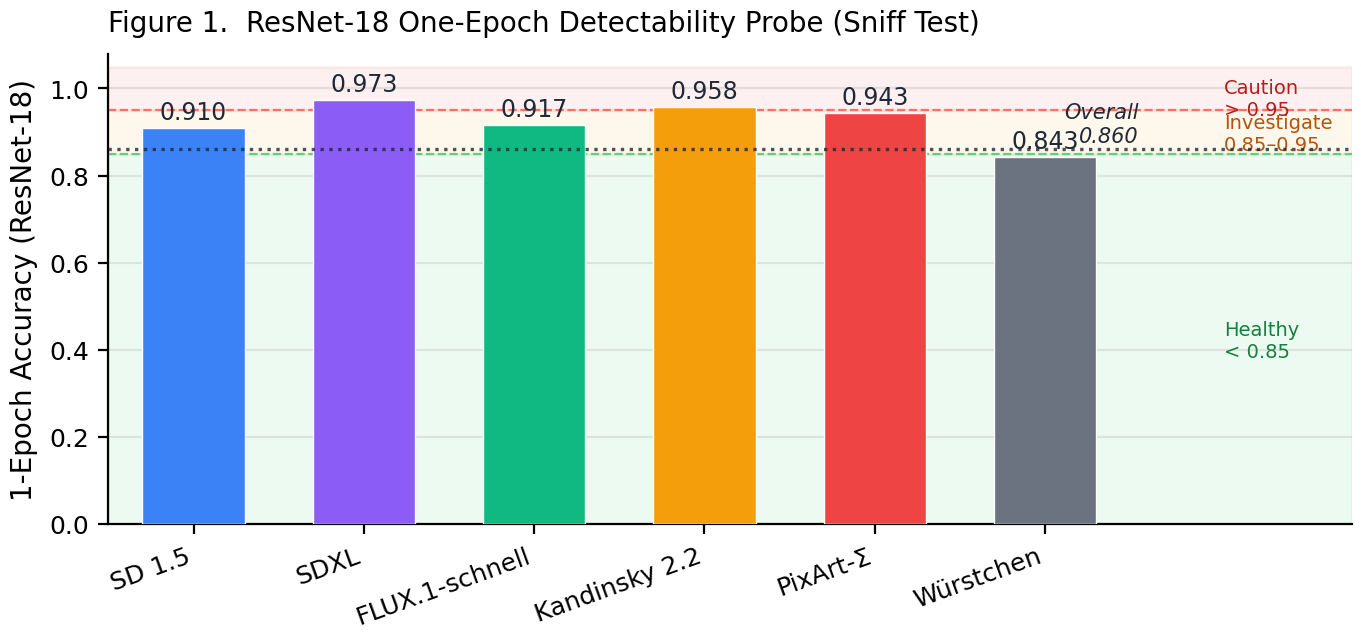
\includegraphics[width=\columnwidth]{fig1_sniff_test.png}
\caption{ResNet-18 one-epoch detectability probe per generator.
Horizontal dashed lines mark the healthy ($< 0.85$) and caution
($> 0.95$) thresholds. The dotted line indicates the overall score
(0.860). W\"{u}rstchen is the only generator in the healthy zone,
consistent with its moderate 42$\times$ latent compression ratio and
the softened artefact profile that compression produces.}
\label{fig:sniff}
\end{figure}

\subsection{Interpreting Sniff-Test Scores}
\label{ssec:sniff_interpret}

Two generators --- SDXL (0.973) and Kandinsky~2.2 (0.958) --- exceed
the caution threshold.
In a dataset that had not applied canonical preprocessing, scores
this high would indicate a compression or resolution leak.
In \textbf{\datasetname}, however, every image has been passed through
the identical JPEG-equalisation pipeline regardless of class label
(Section~\ref{ssec:preprocess}), making a format-based shortcut
structurally impossible.

The elevated scores therefore reflect a genuine property of these
generators: their outputs carry unusually strong and discriminative
synthesis fingerprints that a ResNet-18 can identify in a single
epoch without seeing the full training distribution.
This is consistent with Corvi~\etal~\cite{corvi2023detection},
who showed that different diffusion model architectures produce
qualitatively different artefact profiles in the frequency domain.
The two-stage prior--decoder architecture of Kandinsky~2.2 and the
larger UNet of SDXL both produce rendering characteristics that are
spatially distinctive at the single-epoch probe level.

W\"{u}rstchen (0.843, healthy zone) presents a contrasting profile.
Despite also employing a two-stage hierarchical compression scheme,
its extreme 42$\times$ spatial compression produces a visual output
that a ResNet-18 finds harder to separate from real photographs in a
single epoch.
This is not evidence of better image quality; it is evidence that the
artefacts Würstchen introduces are distributed differently in
frequency space than those of more conventional UNet generators.
The trained EfficientNet-B4 detector (Section~\ref{sec:experiments})
achieves AUROC~$= 0.9745$ on Würstchen images, confirming that the
artefacts are detectable under sufficient training.

The \emph{overall} sniff-test score of 0.860 falls in the investigate
zone, reflecting the architectural diversity of generators rather than
any residual format leak.
The canonical-format audit independently confirms this interpretation:
zero of the 70,000 images fail the \texttt{png\_is\_canonical}
predicate, and no SHA-256 digest mismatches were detected.
The per-generator score variation therefore reflects genuine differences
in synthesis artefact strength across architectural families, not
preprocessing shortcuts.

% ------------------------------------------------------------------
\section{Baseline Experiments}
\label{sec:experiments}
% ------------------------------------------------------------------

We train three standard ImageNet-pretrained classifiers as baseline
detectors on \textbf{\datasetname} and evaluate them on the held-out
test split.
The goal is not to achieve state-of-the-art detection performance,
but to characterise the difficulty landscape of the dataset and
provide reproducible reference numbers against which future work can
be compared.

\subsection{Experimental Setup}
\label{ssec:exp_setup}

\paragraph{Models.}
We evaluate three architectures that span the main families of
modern image classifiers.
\textbf{ResNet-50}~\cite{he2016resnet} is the canonical deep residual
network and the most widely used baseline in the AI-generated image
detection literature~\cite{wang2020cnn,zhu2023genimage}.
\textbf{EfficientNet-B4}~\cite{tan2019efficientnet} is a
compound-scaled convolutional network that achieves substantially
higher accuracy than ResNet-50 at comparable parameter counts.
\textbf{ViT-B/16}~\cite{dosovitskiy2021vit} is a vision transformer
pre-trained on ImageNet-21k and subsequently fine-tuned on ImageNet-1k,
representing the shift from convolutional to attention-based image
encoders.
All models are loaded from the \texttt{timm} library with their
respective \texttt{augreg} or \texttt{ra2} ImageNet checkpoints,
with the final classification head replaced by a two-class linear
layer.

\paragraph{Training.}
Each model is fine-tuned for 10 epochs on the training split
(49,392 images) using AdamW~\cite{loshchilov2019adamw} with a
learning rate of $3 \times 10^{-4}$, weight decay $10^{-4}$, and a
cosine annealing schedule decaying to $3 \times 10^{-6}$.
Gradient norms are clipped to 1.0.
Label smoothing ($\varepsilon = 0.05$) is applied to the
cross-entropy loss to reduce overconfidence.
Training uses a batch size of 64 per GPU across two NVIDIA Tesla T4s
in DataParallel mode.
Data augmentation consists of random horizontal flipping and mild
colour jitter (brightness, contrast, and saturation each varied by
$\pm 0.1$); we deliberately keep augmentation light to avoid
destroying the subtle synthesis artefacts that distinguish generators.
The best checkpoint by validation AUROC is used for test evaluation.

\paragraph{Evaluation metrics.}
We report the area under the ROC curve (AUROC), macro-averaged F1
score, and overall accuracy on the test split (10,486 images).
For per-generator analysis, we compute binary AUROC, F1, and accuracy
on the subset of test images containing the real class paired with
each individual generator (approximately 3,000 images per
generator pair).

\subsection{Overall Results}
\label{ssec:overall_results}

Table~\ref{tab:baselines} and Figure~\ref{fig:overall} present the
overall test-set performance for all three models.

\begin{table}[t]
\centering
\caption{Baseline detector performance on the test split of
\textbf{\datasetname}. All models are ImageNet-pretrained and
fine-tuned for 10 epochs (AdamW, cosine LR, label smoothing
$\varepsilon = 0.05$). Best result per metric in bold.}
\label{tab:baselines}
\begin{tabular}{lccc}
\toprule
Model & AUROC & F1 & Accuracy \\
\midrule
ResNet-50~\cite{he2016resnet}              & 0.7032 & 0.9337 & 0.8757 \\
EfficientNet-B4~\cite{tan2019efficientnet} & \textbf{0.9807} & \textbf{0.9781} & \textbf{0.9614} \\
ViT-B/16~\cite{dosovitskiy2021vit}         & 0.8125 & 0.9310 & 0.8744 \\
\bottomrule
\end{tabular}
\end{table}

\begin{figure}[t]
\centering
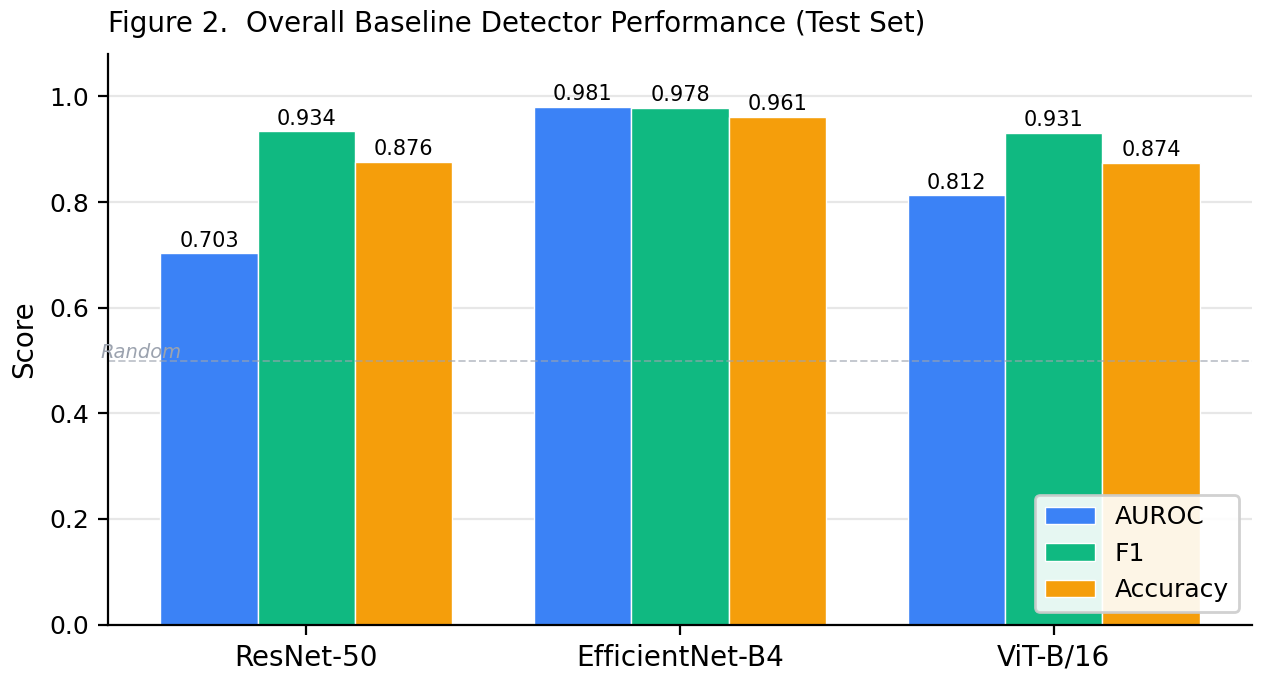
\includegraphics[width=\columnwidth]{fig2_overall_baselines.png}
\caption{AUROC, F1, and accuracy for all three baseline detectors on
the test split. The dashed line at 0.5 indicates chance level.
EfficientNet-B4 dominates on AUROC while ResNet-50 and ViT-B/16
achieve comparable accuracy despite a large AUROC gap, indicating
majority-class defaulting in both.}
\label{fig:overall}
\end{figure}

EfficientNet-B4 achieves the strongest performance across all three
metrics, with an AUROC of 0.9807 and accuracy of 0.9614.
ViT-B/16 occupies a middle ground: its accuracy (0.8744) is close to
ResNet-50 (0.8757), but its AUROC (0.8125) is substantially higher
--- indicating that the ViT produces better-calibrated confidence
scores even where its hard classification decisions are similar to
those of ResNet-50.
The gap between F1 and AUROC is most pronounced for ResNet-50
(F1 of 0.9337 versus AUROC of 0.7032), confirming that ResNet-50
achieves reasonable accuracy by defaulting to the majority class
rather than by reliably separating real from AI images.

\subsection{Per-Generator Analysis}
\label{ssec:per_gen}

Table~\ref{tab:per_gen} and Figure~\ref{fig:heatmap} show the binary
AUROC for the best-performing model (EfficientNet-B4) evaluated
separately for each real-vs-generator pair.

\begin{table}[t]
\centering
\caption{Per-generator binary AUROC on the test split (EfficientNet-B4).
Each row reports classification accuracy on the subset of test images
containing real images paired with the specified generator
($n \approx 3{,}000$ images per pair).
Generators are ordered by increasing AUROC.}
\label{tab:per_gen}
\begin{tabular}{lccc}
\toprule
Generator & AUROC & F1 & Accuracy \\
\midrule
SD~1.5               & 0.9581 & 0.8825 & 0.8728 \\
FLUX.1-schnell       & 0.9734 & 0.8965 & 0.8865 \\
W\"{u}rstchen        & 0.9745 & 0.8965 & 0.8865 \\
SDXL                 & 0.9828 & 0.8991 & 0.8892 \\
Kandinsky~2.2        & 0.9895 & 0.9022 & 0.8922 \\
PixArt-$\Sigma$      & 0.9900 & 0.9041 & 0.8942 \\
\midrule
\textbf{Overall}     & \textbf{0.9807} & \textbf{0.9781} & \textbf{0.9614} \\
\bottomrule
\end{tabular}
\end{table}

\begin{figure}[t]
\centering
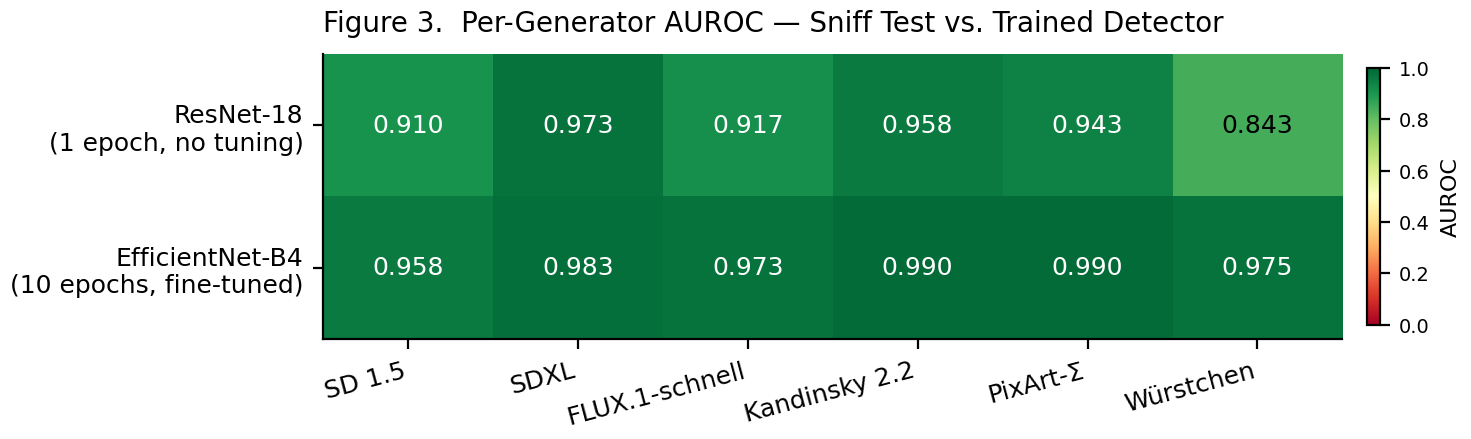
\includegraphics[width=\columnwidth]{fig3_auroc_heatmap.png}
\caption{Per-generator AUROC comparison between the ResNet-18 sniff
test (one epoch, no tuning) and the trained EfficientNet-B4 (10 epochs).
Colour encodes AUROC value from 0 (red) to 1 (green). The sniff-test
row reveals the raw detectability of each generator's artefacts, while
the EfficientNet-B4 row shows what a trained detector can achieve.}
\label{fig:heatmap}
\end{figure}

\begin{figure}[t]
\centering
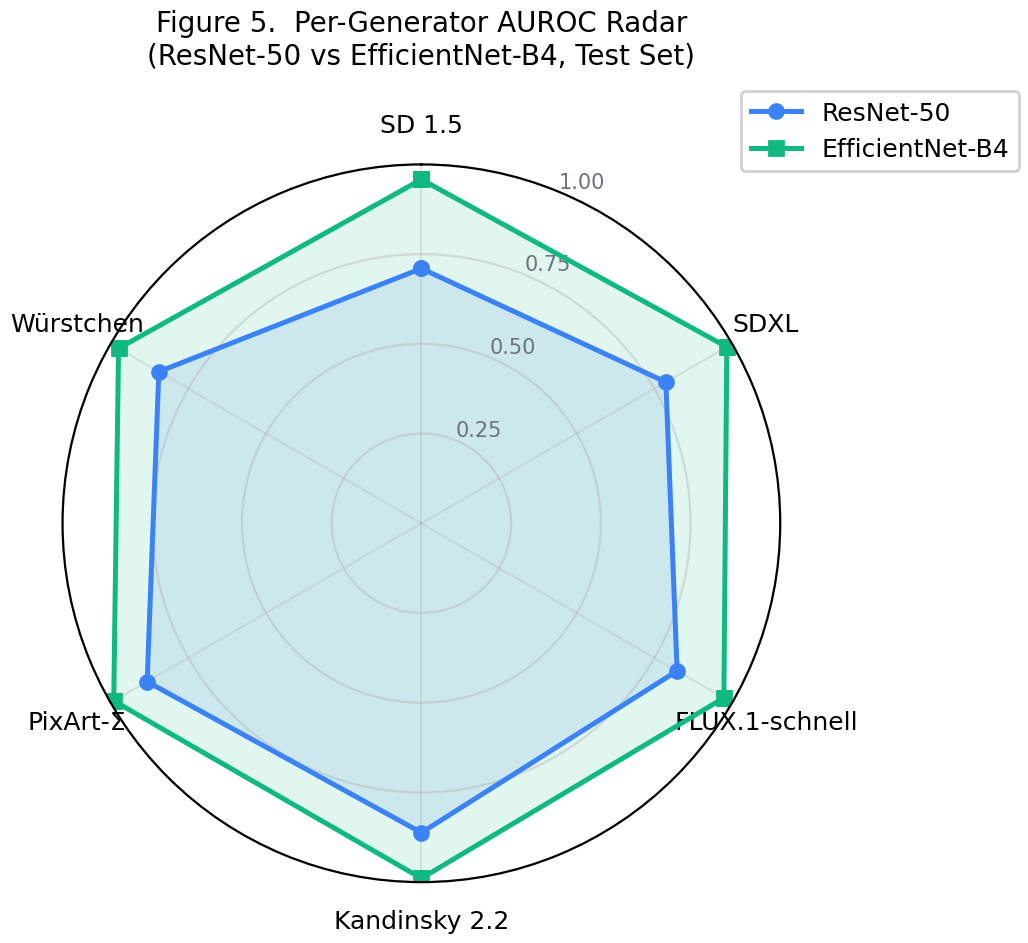
\includegraphics[width=0.75\columnwidth]{fig5_radar.png}
\caption{Radar chart of per-generator AUROC on the test set for
ResNet-50 and EfficientNet-B4.
Note the inward deflection of the ResNet-50 profile on SD~1.5 and SDXL
relative to EfficientNet-B4, confirming that ResNet-50 struggles
disproportionately with UNet-family generators.}
\label{fig:radar}
\end{figure}

All generators are detectable with AUROC above 0.95 by EfficientNet-B4,
but there is a meaningful spread from 0.9581 (SD~1.5) to 0.9900
(PixArt-$\Sigma$).
The radar chart in Figure~\ref{fig:radar} contrasts this per-generator
profile against ResNet-50, making visible the inward deflection of the
ResNet-50 contour on the two UNet generators (SD~1.5 and SDXL).
SD~1.5 remains the hardest generator to detect --- as the oldest and
most widely studied model in the dataset, its artefact profile is
most similar to the general real-image distribution that ImageNet
pretraining has already seen.
W\"{u}rstchen (0.9745) clusters with FLUX.1-schnell (0.9734) just
above SD~1.5, consistent with its healthy sniff-test score and its
highly compressed latent space, which produces artefacts at different
spatial frequencies than UNet-based generators.

All 10,000 W\"{u}rstchen images passed content validation
(pixel standard deviation $> 4.0$), and the per-generator AUROC
of 0.9745 is consistent with the artefact profile expected from
a hierarchical generator operating in a highly compressed latent space.

\subsection{Cross-Generator Generalisation}
\label{ssec:cross_gen}

To evaluate how well a detector trained on known generators can
identify a \emph{previously unseen} generator, we conduct a
leave-one-out (LOO) experiment using ResNet-50.
ResNet-50 is chosen as the LOO backbone because it is the canonical
detection baseline~\cite{wang2020cnn} and because its conservative
discriminative capacity provides a lower-bound estimate of
cross-generator generalisation: a generalisation gap observed under
ResNet-50 is unlikely to be an artefact of an unusually strong
detector.
In each of six runs, one AI generator is held out: the model is
trained on real images paired with the remaining five generators
for five epochs, then evaluated exclusively on real images paired
with the held-out generator (approximately 3{,}000 test images per
run).
Each run is initialised from scratch (no checkpoint reuse across
held-out runs) so that held-out performance reflects genuine
generalisation rather than memorised features.

Table~\ref{tab:cross_gen} and Figure~\ref{fig:crossgen} summarise the
results, grouped by backbone family.

\begin{table}[t]
\centering
\caption{Cross-generator leave-one-out generalisation results
(ResNet-50, 5~epochs per run).
Each row reports AUROC and F1 on the held-out generator's test images
when the model was trained without exposure to that generator.
Generators are grouped by backbone family to make the UNet-vs-non-UNet
divide explicit.}
\label{tab:cross_gen}
\small
\begin{tabular}{lcc}
\toprule
Held-out generator & AUROC & F1 \\
\midrule
\multicolumn{3}{l}{\textit{UNet-based generators}} \\
\quad SD~1.5         & 0.8904 & 0.6672 \\
\quad SDXL           & 0.8609 & 0.6565 \\
\midrule
\multicolumn{3}{l}{\textit{Non-UNet generators (Transformer / Hierarchical)}} \\
\quad FLUX.1-schnell & 0.9586 & 0.8691 \\
\quad W\"{u}rstchen  & 0.9922 & 0.9537 \\
\quad Kandinsky~2.2  & 0.9933 & 0.9678 \\
\quad PixArt-$\Sigma$& 0.9928 & 0.9597 \\
\bottomrule
\end{tabular}
\end{table}

\begin{figure}[t]
\centering
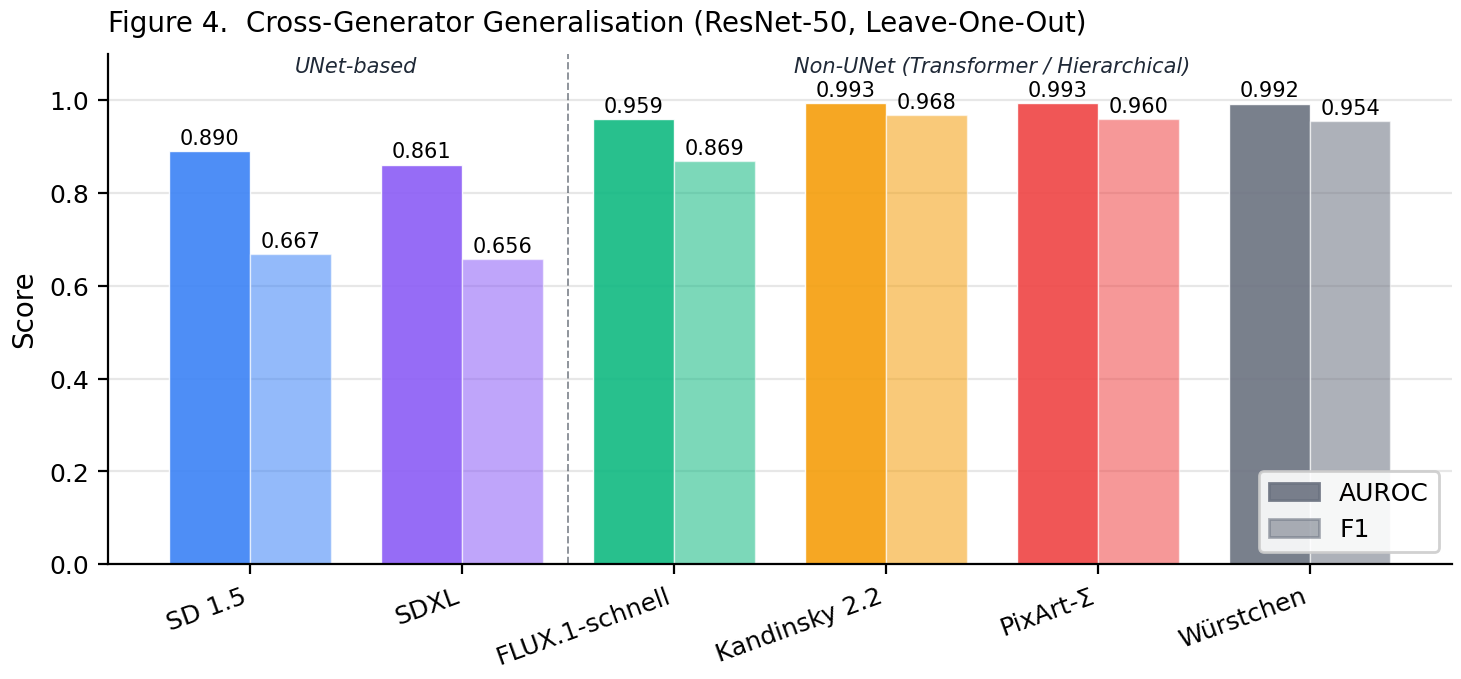
\includegraphics[width=\columnwidth]{fig4_cross_gen.png}
\caption{Cross-generator generalisation AUROC and F1 (ResNet-50,
leave-one-out). Bars share the generator's colour. The vertical dashed
line separates UNet-based generators (left) from
Transformer/hierarchical generators (right). UNet generators are
substantially harder to detect when held out.}
\label{fig:crossgen}
\end{figure}

The results reveal a clean architectural split
(Table~\ref{tab:cross_gen}).

\textbf{UNet generators are the hardest to detect when held out.}
SD~1.5 achieves AUROC~$= 0.890$ and F1~$= 0.667$; SDXL achieves
AUROC~$= 0.861$ and F1~$= 0.657$.
These F1 scores, both below 0.67, indicate that a detector trained
only on non-UNet generators retains limited discriminative signal
for either UNet model.
SD~1.5 and SDXL share the same convolutional UNet architecture and
CLIP-conditioned latent space, so their artefacts are similar enough
that the held-out generator is not fully unseen to the model's
learned representation---but not distinctive enough for
high-precision detection.
This is consistent with WildFake~\cite{hong2024wildfake}, which found
that model architecture is the primary determinant of artefact
structure.

\textbf{Non-UNet generators are near-perfectly detectable when held out.}
W\"{u}rstchen (0.992), Kandinsky~2.2 (0.993), and PixArt-$\Sigma$
(0.993) all exceed AUROC~$= 0.992$, with F1 scores above 0.95.
This indicates that Transformer and hierarchical architectures produce
artefacts so qualitatively distinct---both from real images and from
UNet synthesis patterns---that a detector identifies their outputs as
anomalous without having seen them during training.
FLUX.1-schnell occupies an intermediate position
(AUROC~$= 0.959$, F1~$= 0.869$), consistent with its few-step
distillation regime producing artefacts closer in character to real
photographs than full-step Transformer models.

\textbf{\datasetname} is the first publicly available paired dataset
to include both architectural families simultaneously under identical
preprocessing conditions, making this cross-family comparison
structurally possible for the first time.

% ------------------------------------------------------------------
% BIBLIOGRAPHY ADDITIONS
% ------------------------------------------------------------------
